\documentclass{article}
\setlength{\parskip}{0pt} % esp. entre parrafos
\setlength{\parindent}{20pt} % esp. al inicio de un parrafo
\usepackage{amsmath} % mates
\usepackage{listings}
\usepackage{xcolor}
\usepackage[sort&compress,numbers]{natbib} % referencias
\usepackage{url} % que las URLs se vean lindos
\usepackage[top=10mm,left=20mm,right=20mm,bottom=25mm]{geometry} % \textbf{\textbf{}}margenes
\usepackage{hyperref} % ligas de URLs
\usepackage{graphicx} % poner figuras
\usepackage{caption}
\usepackage{subcaption}
\usepackage[spanish]{babel} % otros idiomas
\hypersetup{
    colorlinks=true,
    linkcolor=blue,
    filecolor=blue,      
    urlcolor=blue,
}
\renewcommand{\lstlistingname}{Código}
\definecolor{codeblack}{rgb}{0,0.6,0}
\definecolor{codegray}{rgb}{0.5,0.5,0.5}
\definecolor{codepurple}{rgb}{0.58,0,0.82}
\definecolor{backcolour}{rgb}{0.95,0.95,0.92}
\lstdefinestyle{mystyle}{
    backgroundcolor=\color{backcolour},   
    commentstyle=\color{codeblack},
    keywordstyle=\color{blue},
    numberstyle=\tiny\color{codegray},
    stringstyle=\color{codeblack},
    basicstyle=\ttfamily\footnotesize,
    breakatwhitespace=false,         
    breaklines=true,                 
    keepspaces=true,                 
    numbers=left,                    
    numbersep=5pt,                  
    showspaces=false,                
    showstringspaces=false,
    showtabs=false,                  
    tabsize=2
}
\lstset{style=mystyle}

\title{"P6" Sistema Multiagente}
\author{NESTOR}
\date {Marzo 2022}

\begin{document}

\maketitle

\section{Objetivo}
El objetivo de esta actividad es el implementar un sistema multiagente con una aplicación en epidemiología. Los agentes podrán estar en uno de tres estados: susceptibles, infectados ó recuperados esto se conoce como el modelo SIR. \cite{elisa1}.

\section{Desarrollo}
El desarrollo de la actividad esta basado en el \href{https://https://https://satuelisa.github.io/simulation/p6.html}{c\'odigo} implementado por E. Schaeffer \cite{elisa1}. Basando el desarrollo, en el código \cite{elisa1} se establecen las instrucciones para la ejecución del programa. Se encuentra todas las instrucciones en el  \href{https://https://https://github.com/NestorZeus/SIMULACION-COMPUTACIONAL-DE-NANOMATERIALES/tree/main/P6}{repositorio} de Nestor en GitHub.\\

\begin{lstlisting}[caption=Ejecución de Parámetros, label=codigo1, language=Python]
import seaborn as sns
from math import floor, log, sqrt
from random import random, uniform
from time import time
from scipy.stats import f_oneway
import pandas as pd
import matplotlib.pyplot as plt
n = 40
pi = 0.09
pr = 0.05
\end{lstlisting}

Ejecutando con la función, se genera una cantidad de numeros de contagios aleatorios. Esto se define un conjunto de funciones que se utilizan. Los parámetros serán el número de contagios  y la probabilidad de posibles contagios. La probabilidad de contagio será en nuestro caso proporcional a la distancia euclideana entre dos agentes  de la siguiente manera de la ecuación:

\begin{equation}\label{eq1}
    p_c =
    \begin{cases}
    0\text{,} & \text{si} \ d(i,j) \geq r\text{,}\\
    \frac{r-d}{r}\text{,} & \text{en otro caso,}
    \end{cases}
\end{equation}

\begin{lstlisting}[caption= Instrucciones para generar parámetros epidemiológicos infectados, label=codigo3, language=Python]
def contagiados():
 for i in range(n):
  a1 = agentes.iloc[i]
  if n < 1:
  return True
  for i in range(2, n):
  if n % i == 0:
  return False
  if d < r:
  if random() < (r - d) / r:
  contagios[j] = True
  return contagios
\end{lstlisting}


Para saber el programa de como se genera el cuadro que se llama las funciones y se pueda generar, \href{https://https://satuelisa.github.io/simulation/p6.html} implementados por E. Schaeffer, se muestra a continuación en el código \ref{codigo3}. Los agentes tendrán coordenadas  y una dirección y una velocidad. Se ejecutará los parámetros a posicionar. \cite{elisa1}

\begin{lstlisting}[caption= Instrucción para generar agentes, label=codigo4, language=Python]
for k in range(runs):
    agentes =  pd.DataFrame()
    agentes['x'] = [uniform(0, l) for i in range(n)]
    agentes['y'] = [uniform(0, l) for i in range(n)]
     x = a.x + a.dx
\end{lstlisting}

Se ejecuta los parámetros para una serie de probabilidades de epidemias y contagios, para representar los resultados. 

\begin{lstlisting}[caption= Resultados de epidemias y contagios, label=codigo4, language=Python]
epidemia = []
    for tiempo in range(tmax):
    conteos = agentes.estado.value_counts()
    infectados = conteos.get('I', 0)
    epidemia.append(infectados)
    contagios = [False for i in range(n)]
\end{lstlisting}

Se ejecuta los parámetros para una serie de probabilidades de Pico más alto y Caso sospechosos, para representar los resultados.

\begin{lstlisting}[caption= Resultados de Pico más alto y Caso sospechosos, label=codigo4, language=Python]
elif a.estado == 'I':
    if random() < pr:
    agentes.at[i, 'estado'] = 'R'
    x = a.x + a.dx
    y = a.y + a.dy
    x = x if x < l else x - l
    y = y if y < l else y - l
    x = x if x > 0 else x + l
    y = y if y > 0 else y + l
    agentes.at[i, 'x'] = x
    agentes.at[i, 'y'] = y
    maximos['Pico más alto'].append(max(epidemia))
    maximos['Caso sospechosos'].append(epidemia.index(max(epidemia)) + 1)

\end{lstlisting}

\section{Resultados}\label{res}
En los diagramas se representa como es el comportamiento de los resultados de infectados, pico de infectados, casos sospechosos y disminución de casos. Las variaciones no hay una estadística perfecta para comparar el impacto de la pandemia. Una combinación de diferentes métricas puede ofrecer una visión más completa del impacto del virus. Estas gráficas representan distintas estadísticas, cada una con sus propias fortalezas y debilidades.

\newpage
\begin{figure}
    \centering
    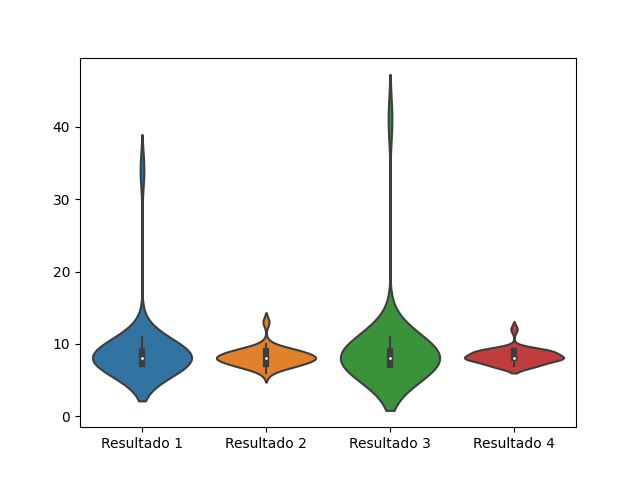
\includegraphics[width=100mm]{Figure_1.png}
    \caption{Diagrama de infectados, pico de infectados, casos sospechosos y disminución de casos}
    \label{figure}
\end{figure}

\begin{figure}
    \centering
    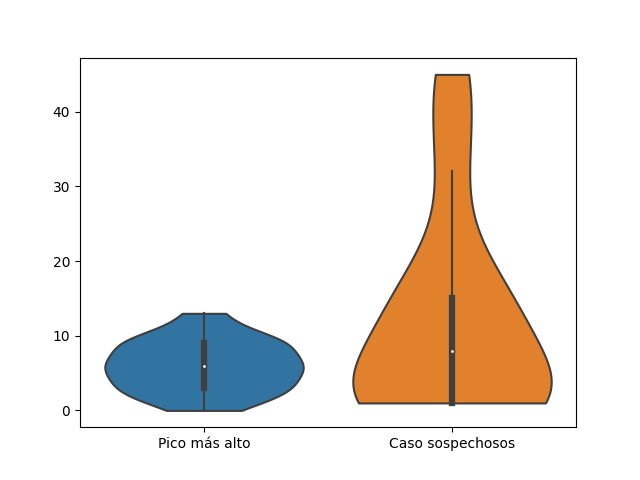
\includegraphics[width=95mm]{Figure_2.png}
    \caption{Diagrama de pico más alto infectados y casos sospechosos}
    \label{figure}
\end{figure}

\section{Conclusiones}
Se concluye que se reporta los datos de forma ligeramente distinta y de forma inevitable ya que no han sido diagnosticados. A medida que estos tratan de contener la propagación del virus, independientemente de si se están acercando o ya pasaron el pico de contagios, o si están experimentando un resurgir de contagios.


\bibliographystyle{plainnat}
\bibliography{simulacion}

\cite{elisa1}
\cite{2}
\end{document}
